\section{Introduction}\label{sec:intro}

Although deep learning has gained enormous success, it requires huge amounts of data for training, and its black-box characteristics regarding decision criteria result in a lack of reliability. For example, CLIP {\cite{CLIP} needs 400 million image pairs for training and Stable Diffusion XL (SDXL) {\cite{SDXL} requires 5 billion images. This implies only a small number of groups can train foundation models from scratch. Also, the black-box nature makes it hard to anticipate the model’s performance in different environments. For example, suppose we are to classify pictures of deer and most training deer images contain antlers. For the test images taken in winter,  %How would the performance be? 
the performance will be worse as deer shed their antlers in winter. %if the model classifies \nj{the presence} of deer with antler. 
As modern deep learning models do not provide any decision criterion \ie black box, \jh{we} cannot determine whether the domain of the model has shifted, or if the model is biased in advance, thus cannot anticipate the performance drop in this case.

Interestingly, these problems do not occur in previous state-of-the-art, support vector machines (SVMs), which require substantially less data, enabling almost anyone to train a model from scratch. Also, as it encodes the decision boundary explicitly, SVM can reconstruct the support vectors from the training dataset using the KKT condition. %, which is the decision criterion.} 
Since it %has an explicit criterion,
is a white box, one can anticipate the test’s performance in advance.  In the deer classification example, if the model’s support vectors of deer have prominent antlers, using that SVM is not appropriate for photos taken in winter. 
%Furthermore, SVM's characteristics enable the reconstruction of data using the decision boundary itself.

In this paper, we tackle the natural limitations of deep learning -- the need for large data and black-box characteristics -- by extracting SVM features in deep learning models. In doing so, we introduce the DeepKKT condition for deep models, which corresponds to the KKT condition in traditional SVMs. By either selecting deep support vectors (DSVs) from training data or generating them from already trained deep learning models,
%without train data using logits as latents}. \jh{Our solution does not require any restrictions on the type of deep learning model.} %\nj{In doing so, we introduce} the DeepKKT condition, which \nj{corresponds to} a KKT condition for deep learning models. 
we show DSVs can play a similar role to conventional support vectors. Like support vectors can reconstruct SVM, we can reconstruct the deep models from scratch only with DSVs. Also, we show that DSVs encode the decision criterion visually, providing a global explanation for the trained deep model.
\nj{Expanding beyond conventional support vectors, DSVs suggest that a trained deep classification model can also function as a latent generative model by utilizing logits as latent variables and applying DeepKKT conditions.}
%\jh{Expanding beyond from conventional support vectors, DSVs propose that a trained deep classification model can also function as a latent generation model by utilizing logits as latent variables and applying DeepKKT conditions.}
% \jh{Expanding further from SVM, we suggest that a trained deep classification model can also function as a latent generation model by utilizing logits as latent variables and applying DeepKKT conditions.}
%\jh{Furthermore, we \nj{give a hint} that \nj{a trained deep classification model} can serve as \nj{a latent generation model} with DeepKKT conditions by using logits as latent.}



To this end, we generalize the KKT condition and define the DeepKKT condition considering that the data handled by a deep model is high-dimensional and multi-class. 
We demonstrate that the selected data points (selected DSVs) among the training data satisfying the DeepKKT condition are closer to the decision boundary than other training data, as evidenced by comparing entropy values.
%We show that when a set satisfying the DeepKKT condition is extracted from the original training set \nj{(selected DSVs)}, this set is closer to the decision boundary compared to other data by comparing entropy. 
Also, we show that the calculated Lagrangian multiplier can reveal the level of uncertainty of the model for the sample in question. %which class the model finds difficult to predict. 
%Moreover, when generating data that meets the DeepKKT condition (synthesized DSVs), we confirm that they contain as much information as the original training data.
Additionally, we demonstrate that the  DSVs outperform existing algorithms in the few-shot dataset distillation setting, where only a portion of the training set is used, indicating that DSVs exhibit characteristics similar to SVMs. Moreover, we confirm that modifying existing images using information obtained from DSVs allows us to change their class at will, verifying that DSVs can meaningfully explain the decision boundary. Finally, by using soft labels as latent variables in ImageNet, we generate unseen images with high fidelity.

%Additionally, \nj{we show that the generated DSVs result in} better performance than existing algorithms in the few-shot dataset distillation setting, where only a part of the training set is used, \jh{thus showing it serve as similar characteristics to SVM}. and we confirmed that modifying existing images using the information obtained through DSVs can \nj{change the class at our will}, verifying that DSVs can meaningfully explain the decision boundary. Finally, we generated unseen images with high fidelity by using soft labels as latent in imagenet.

Our contributions are as follows:

\begin{itemize}[leftmargin=*]
    \item By generalizing the KKT condition for deep models, we propose the DeepKKT condition to extract Deep Support Vectors, which are applicable to general architectures such as ConvNet and ResNet.
    \item We verify that DeepKKT can be used to extract and generate DSVs for common image datasets such as CIFAR10, CIFAR100, SVHN, and ImageNet.
    \item DSVs are better than existing algorithms in few-shot dataset distillation problems. %compared to existing algorithms.
    \item \jh{DeepKKT acts as a novel model inversion algorithm that can be applied in practical situations.}
    \item By using the DeepKKT condition, we not only show the trained deep models can reconstruct data, but also can serve as latent generative models by using logits as latent.
\end{itemize}

% IE 만들기
% \begin{figure}[t]
%   \centering
%    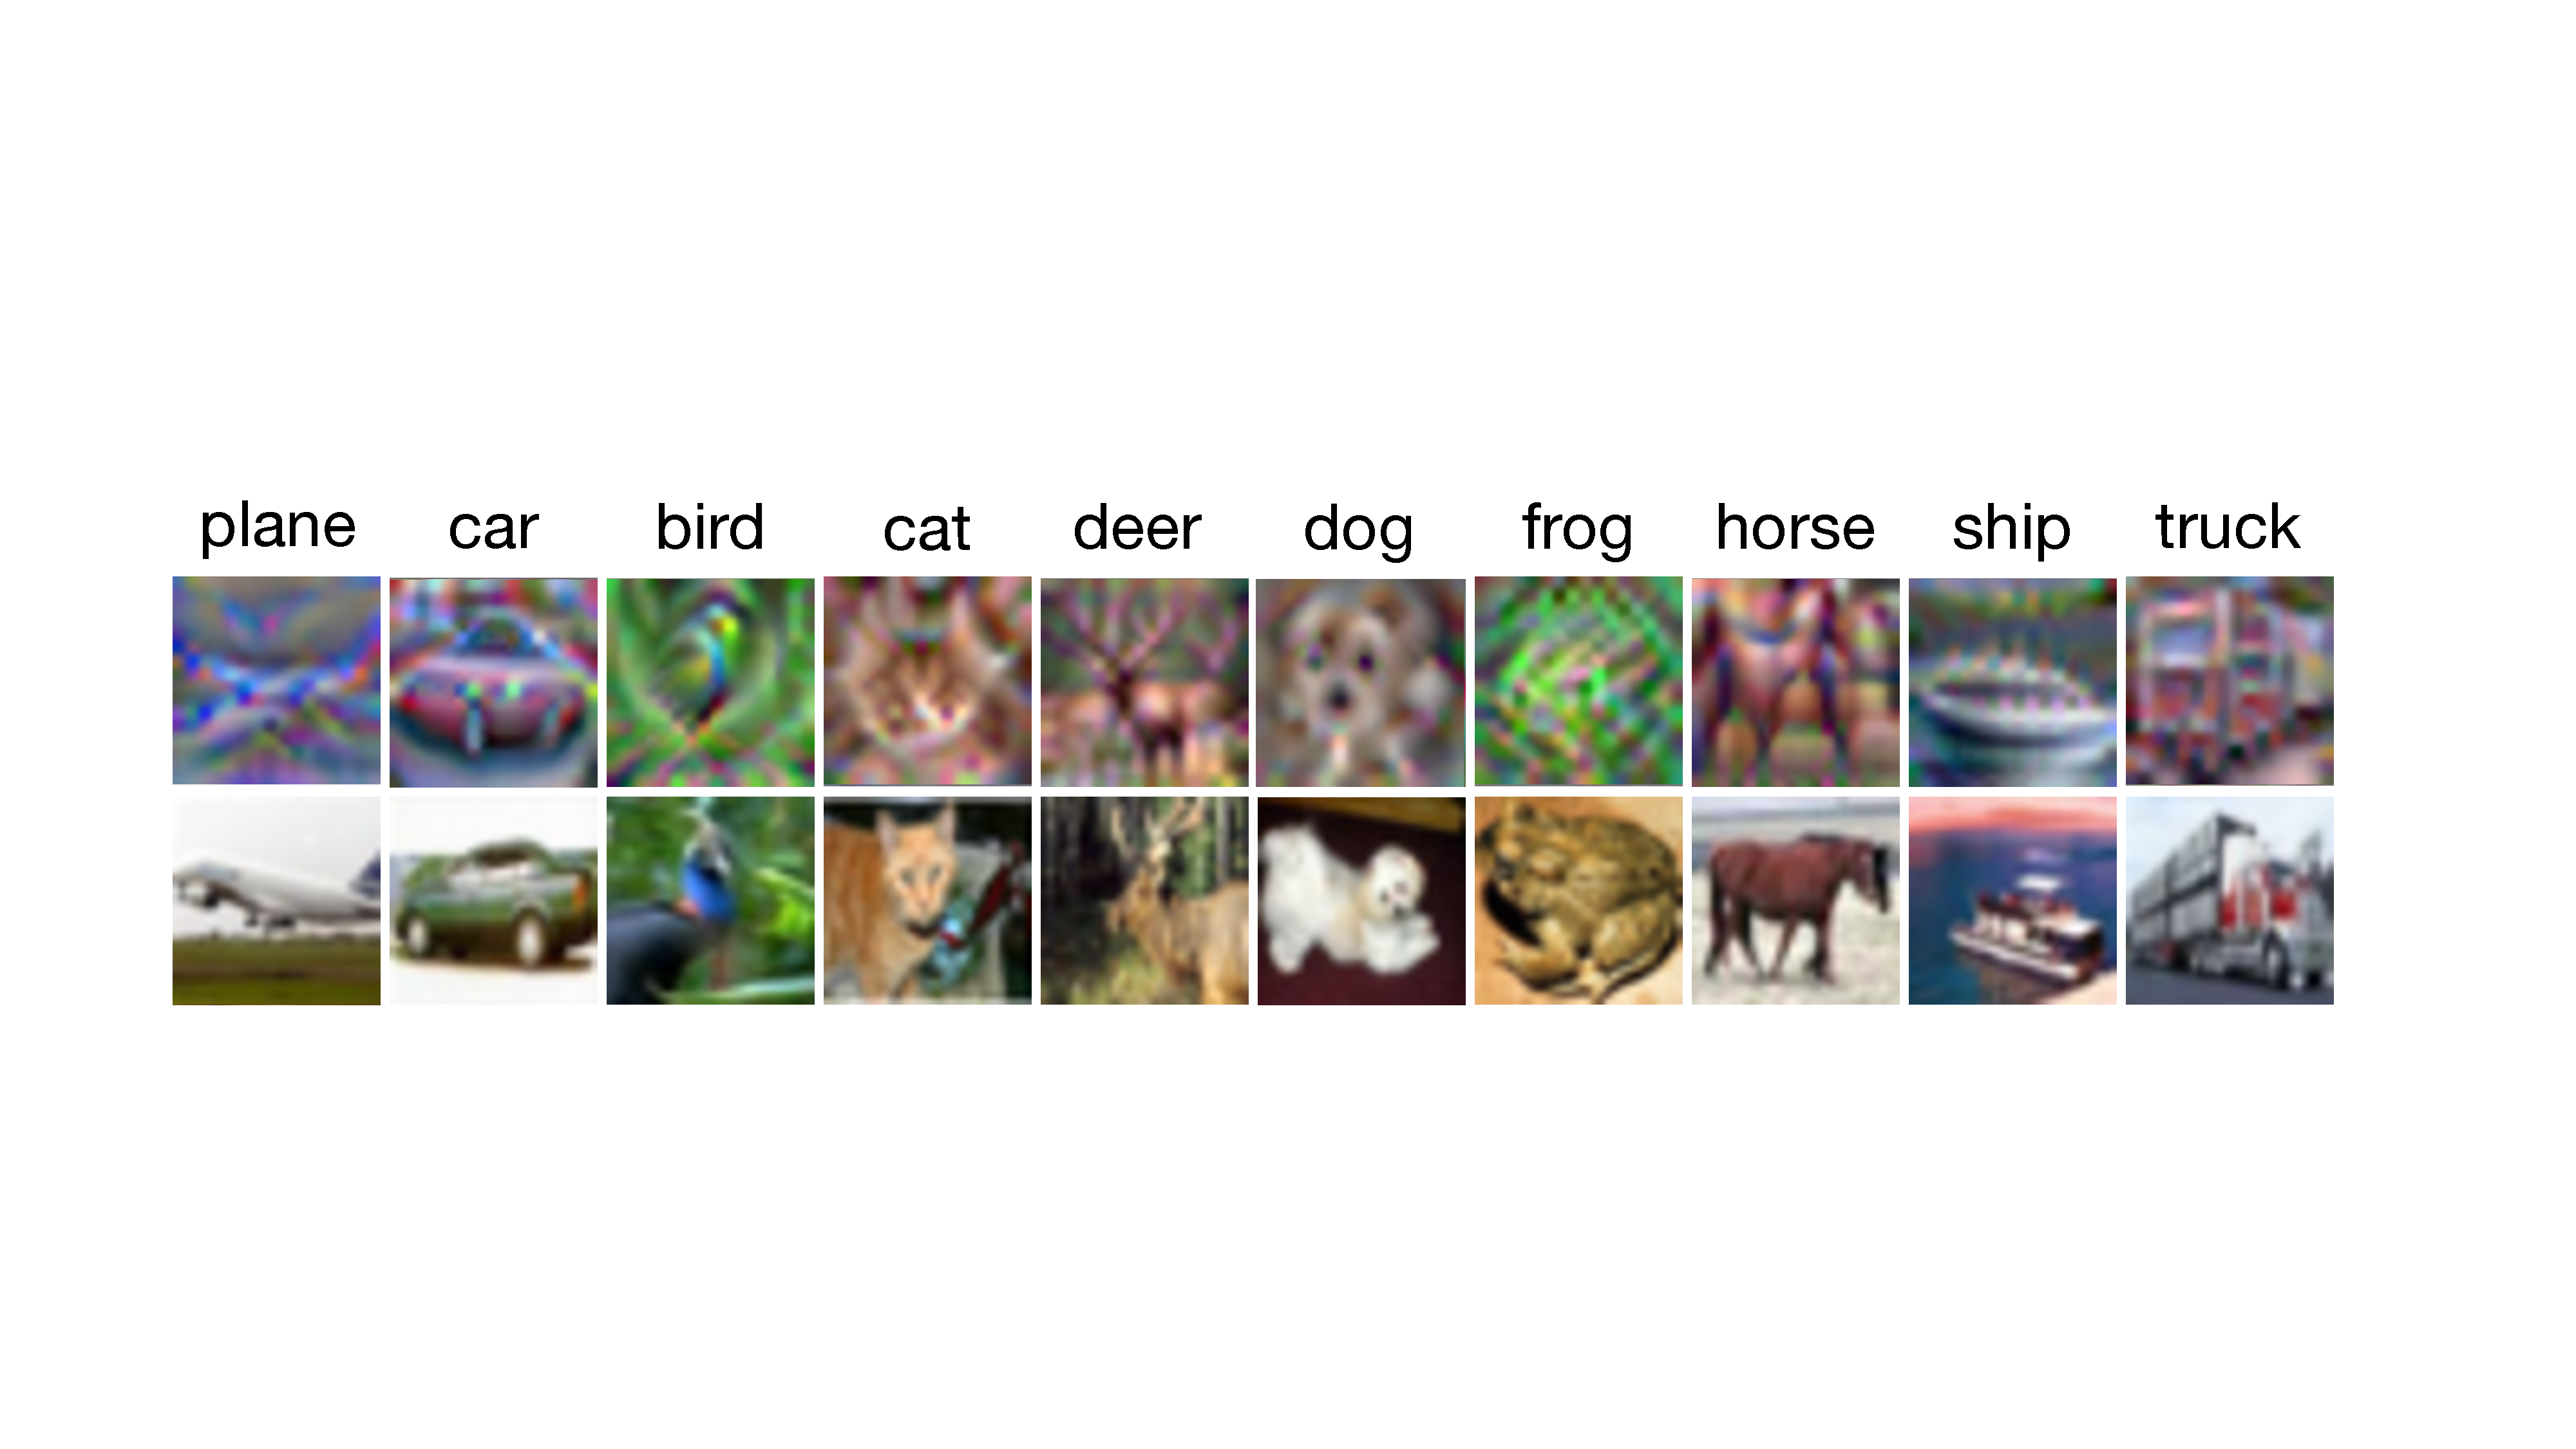
\includegraphics[width=1.0\linewidth]{./figure/dsvset.pdf}
%    % \includegraphics[width=0.8\linewidth]{author-kit-CVPR2024-v2/figure/manifoldfigure.pdf}
%    \caption{Comparison of synthesized images (first row) created using the DeepKKT condition initiated from noise, and selected images (second row) from the CIFAR-10 training dataset. The selected images were chosen based on \nj{$\lambda$} values, \nj{\ie each image has} the highest \nj{$\lambda$} in each class. Both synthesized and selected images demonstrate similarity at the pixel level sharing common features.}
%    \label{fig:DSVSET}
% \end{figure}
% 딥러닝은 좋지만, 이것의 내부 과정에서 decision criterion을 알 수 없다는 black-box characteristics 때문은 이것의 application을 성능 측면에서, reliability 측면에서 apply하게 어렵게 만든다. 예를 들어서 우리가 분류 모델을 하나 들이려고 하느데, 이때 우리가 분류해야할 사슴 사진이 겨울에 찍혔다고 하자. 그렇다면 우리는 해당 사진을 일반적인 사슴이 분류에 있는 분류 모델을 들고오면 다 되는걸까? 또한, 이런 black-box characteristics는 reliability 문제를 야기한다. 과연 성능만 높으면 되는걸까? 예를 들어서 어떤 모델이 얼굴 사진을 가지고 와서, 그 사진에 대해서 수염의 여부를 측정한다고 해보자. 만약 그것의 accuracy가 높다고 하면, 우리가 과연 그것을 믿을 수 있을까? 예를 들어서 단순히 남자임을 측정하여서 그렇게 문제를 풀지는 않을까? 이 경우에 우리는 그 모델을 믿을 수 없을 것이다. 또한 딥러닝은 좋은 성질을 가지고 있지만, 격차를 벌린다는 단점이 있다. 시간이 가면 갈수록 , 딥러닝은 expotential하게 많은 데이터를 학습시키기 위해서 요구하고, 결국에는 computation 자원이 넉넉한 몇개의 집단만 그것을 활용가능하게 만들었다.

% 흥미롭게도, 90s ~ 00s 딥러닝 이전 최고의 AI였던 classical ML은, 사슴 문제와 수염 문제, 그리고 data resource 문제에 대해서 자유로웠다는 것이다. 예를 들어 90년대와 00년대 당시 최고의 성능을 기록하였던건 SVM인데, 이것의 경우는 전체 데이터셋에서 분류 margin을 최대화하는 support vector들을 뽑아서 이것들을 decision criterion으로 활용하였다. 이 모델의 경우는 위의 사슴 문제와 수염 문제를 풀 수 잇다. 단순히 support vector들을 보았을 때, 사슴을 구분하는 criterion인 support vector에서 뿔이 두드러지게 나타나 있다면, 우리는 그 모델을 쓰지 않는것이 좋다. 왜냐하면 이는 모델이 사슴의 뿔을 기준으로 판단한다는것을 암시하는데, 사슴은 겨울에 뿔갈이를 하기 때문에 뿔이 없기 때문이다. 비슷하게, support vector, 그리고 근처의 image들이 다 수염을 기른 남성이라면, 우리는 어느정도 그 모델은 bias되어 있다고 판단할 수 있다. 또한, Classical ML의 경우는 데이터셋을 크게 요구하지 않는다. 

% 위해서 열거한 문제를 해결하기 위해서 기존에 다양한 방법으로 문제를 해결하곤 하였다. XAI, Debiasing, Dataset Distillation. 그리고 SVM architecture를 들고오는 것

% In this paper, 우리는 딥러닝에 산재한 문제들을, 가장 자연스러운 방법으로 해결하였다. 우리는 '처음으로',Specifically, DeepKKT condition, which is generalization of KKT ocndition + manifold hypothethis,We have shown DSVs have similar property to conventional SVM,  어떤 종류의 trained model에서, Corresponding Support vector, 기존의 수많은 시도들이 존재하였으나, 이것들은 전부 다 SVM architecture 자체를 딥러닝에다가 옮기려고 한 것. 우리는 어떤 종류의 수정도 가하지 않음. 우리는 가장 '일반적'이라고 가정되는 architecture - augmented, small-batch, any architecture - Various Domain. Show property

% Measuring lambda, Prediction, Dataset distillation with DSVs, measured Debias, 


% 시작 인트로: 2010년대 중반부터 시작된 딥 러닝은 뭐 엄청 잘 되고, 이런 분야부터 저런 분야까지, 뭐 그냥 잘 된다. 당연한 수순으로, 딥 러닝이 왜 잘 돌아가는지 연구도 활발하게 되고 있는데, 이를 설명하는데 있어서 딥 러닝을 기존의 well-defined된 classicial machine learning으로 연결지어 해석하기도 한다. 그 중에 가장 promising 한 방법은 Deep learning과 Kernel method를 연관짓는 방법론이며, 딥 러닝의 모델은 이미 overparameterized regime일 때 Kernel method와 등가인 것은 널리 알려진 사실이다. 또한, 이런 overparmeterized 상황에서 딥 러닝 모델은 kernel method를 활용한 방법 중 하나인 support vector machine (SVM)과 같게 움직이는 것이 알려져 있는데, 기존의 상황에서는 등가임만 증명하였고, 그것이 실제로 어떤 형식으로 support vector가 되는지는 설명되지 않았다.


% DL이 왜 patten generalization 분야에서 좋은 성능을 내는지, 또한 어떤 과정을 통해서 DL이 판단하는지에 대한 이해가 부족하다는 어두운 면이 있다.

% 이러한 면을 해결하기 위하여, 가장 major한 분야는 이미 well-defined 된 eclassicial machinie learning로 끌어와 설명하는 것이다. 
% 특히 SVM과 연관지어서 설명하는 경우가 많은데, 실제로 이게 특정 조건에서 성립하기도 할 뿐더러 SVM 자체는 굉장히 좋은 properties를 가지고 있기 때문이다. 첫째, SVM은 
% 굉장히 잘 연구되어지고, 왜 잘 작동하는지에 대한 이론적인 연구가 잘 되어 있다. 둘째로, 학습된 SVM 모델 자체는 매우 좋은 interpretability를 가지고 있기 때문이다.
% 예를 들어 SVM 모델만 가지고 있다고 하더라도, 우리는 그 모델만 가지고 support vector를 어느정도 구할 수 있으며, 구한 support vector들로 그 machine이 어떤 기준을 가지고
% unknown data를 판단하는 지에 대한 insight를 얻을 수 있기 때문이다.

% 만약 그렇다면, Deep learning model에서 SVM과의 equivalence를 보인 시점에서 다음과 같은 질문은 자연스럽다. 과연 우리는 DL에서도 SVM에서의 support vector에 해당하는, Deep Support Vector (DSV)를 찾을 수 있을까?
% 하지만, 어떤 논문도 conventional deep learning 모델에서 직접적으로 support vector를 찾지 못했는데, 그 이유는 다음과 같은 어려움 때문이다 첫째로, SVM과 DL은 철학이 다르다. SVM의 철학을 요약하자면
% 오컴의 면도날과 같다고 할 수 있다. 같은 성능을 낸다면, 더 적은 파라미터를 쓰는 것이 좋다. 하지만 DL의 경우, overparameterized region에서 overfitting하는 것이 핵심이기에, 직접적인
% equivlaence를 찾기 어렵다는 단점이 있다. 둘째로, DL이 주로 다루는 input은 high-dimensional parameter space이기 때문에, 실제로 그 space에서 data가 차지하는 manifold는 계속 작아진다.

% 따라서, 우리가 support vector를 찾기 위해서 parameter space에서 optimize 한다면, 그것을 만족하는 해가 실제로 data manifold에 존재할 확률이 낮아진다는 점이다.

% - 본 논문의 첫 파트에서, 우리는 그 문제에 대해서 도전한다.
%  Under mild assumptions, we show that support vector exists, and we can
% - derive support vector from the trained model. Without any access to training dataset. 
% - To do so, we first show that support vectors exists by revisiting the dynamics of conventional loss function which has expotential tail. 
% - Then, derive some necessary condition that support vector should satisfy. 
% - Finally, we argue that obtained support vectors is not sufficient due to curse of dimensionality, it is high likely to be outside of data manifold.
% - To enforce it lie in data manifold, we adopt lie algebraic approach to obtain support vecor which lie in data manifold. By enforcing support vector satisfy
% - lie equivalence, we can obtain support vector which lie in data manifold.

% - Second part is the catalog of support vector. We show that subtracted support vector has some interesting properties.
% - We show that deep support vector (DSV) can be interpreted as solving dataset condensation problem with harsh condition.
% - i.e., dataset condenstation without having real dataset with single trained model. 
% - Also, we can view DSV as global explanation in XAI. As DSV is obtained without any access to real dataset.
% - Each class of DSV is reprensatitive of each class. DSV provides global insight of the model on how model
% - classifyes the data.
% - Finally, we show that DSV can be used as global adversal patch from which obtained without any access to real dataset.

% 딥러닝은 현대 기술의 획기적인 진전을 이끌며 많은 분야에서 혁명을 일으켰습니다. 그러나 이러한 성공에도 불구하고, 딥러닝 모델이 패턴 일반화에서 어떻게 뛰어난 성능을 발휘하는지, 또한 모델이 어떠한 기준으로 판단하는지에 대한 근본적인 이해는 아직 부족한 상태입니다. 이 연구는 딥러닝의 블랙박스를 해체하고, 이러한 모델이 데이터를 어떻게 처리하고 해석하는지에 대한 더 깊은 이해를 제공하기 위한 시도입니다.

% 이 연구의 첫 번째 목표는, 고전적인 머신러닝 방법인 서포트 벡터 머신(SVM)과 딥러닝 간의 관계를 탐색하는 것입니다. SVM은 그 해석 가능성과 잘 정립된 이론적 배경으로 잘 알려져 있습니다. 이러한 특성은 우리가 모델에서 서포트 벡터를 추출하고, 이를 통해 모델이 어떻게 미지의 데이터를 분류하는지에 대한 통찰력을 제공합니다. 이 연구에서는 이러한 서포트 벡터의 딥러닝 버전, 즉 딥 서포트 벡터(DSV)를 정의한 다음, 그 존재를 증명하고 이를 추출하는 방법을 제시합니다.

% 왜 novel한지에 대한 section을 만들기.

% 두 번째 목표는 DSV가 실제 세계 문제에 어떻게 적용될 수 있는지를 탐구하는 것입니다. DSV를 사용하면 데이터 셋 축소 문제를 해결할 수 있으며, 실제 데이터 세트에 대한 접근 없이도 전역적인 설명 가능성을 제공할 수 있습니다. 또한, DSV는 각 클래스를 대표하는 특징을 제공함으로써 모델이 데이터를 어떻게 분류하는지에 대한 전역적인 통찰력을 제공합니다.

% 본 논문은 먼저, 일반적인 손실 함수의 역학을 재검토함으로써 서포트 벡터의 존재를 보여줍니다. 그 후, 서포트 벡터가 충족해야 할 필요 조건을 도출하고, 차원의 저주로 인해 얻은 서포트 벡터가 데이터 매니폴드 외부에 있을 가능성이 높다는 것을 논의합니다. 이를 해결하기 위해, 데이터 매니폴드 내에 있는 서포트 벡터를 얻기 위한 리 대수적 접근법을 채택합니다.

% 그 다음, 본 연구는 우리가 정의하고, 구한 DSV가 어떤 가능성이 있는지 소개합니다. 먼저, DSV가 가진 support vector로서의 측면에서, DSV가 Dataset Condensation 문제를 해결할 수 있음을 시사합니다.  그 다음, DSV를 통하여 기존에 불가능했던 Explainable AI의 Global explanation 기능을 제공할 수 있음을 시작합니다. 마지막으로, DSV가 training dataset에 대한 접근을 하지 않고 생성한 Global Adversarial attack problem을 해결할 수 있음을 보여줍니다.

% 이 연구는 딥러닝의 해석 가능성과 일반화에 대한 우리의 이해를 향상시키는데 중요한 첫 걸음이 될 것입니다. 또한, 본 연구를 통해 제시된 방법론과 발견들은 딥러닝 모델의 설명 가능성과 신뢰성을 향상시키는 데 기여할 것입니다.

% Deep learning has led revolutionary advancements in modern technology, catalyzing paradigm shifts across numerous fields. However, despite these successes, a fundamental understanding of how deep learning models excel in pattern generalization and the criteria they use for decision making remains uncertain. This research endeavors to demystify the black box of deep learning, offering deeper insights into how these models process and interpret data.

% % \jh{SVM의 성질에 대한 시도를 넣어야 한다. 그러니까 Decision boundary의 coordinate 역할을 한다 뭐 이런거 기존 가지고 성질을 설명하면서, 그것의 high level에서의 정의. 간단하게 언급하고, 그 다음에 렐웍에다가 넣든지 하자.}

% In explaining the performance of deep learning, one of the most useful attempts is associating it with \textit{support vector machines} (SVM) \cite{SVM_vapnik, SVM_original_paper} 
% %\nj{vapnik cortes의 original paper를 같이 인용할 것!} 
% because SVM theoretically provides a well-tight bound on its performance. Consequently, support vectors, which encode the decision boundary, offer valuable insights into how the model classifies based on certain criteria. Moreover, the number of support vectors is much smaller than the size of the trained dataset, making it parameter-efficient. This idea aligns well with deep learning models that converge to 100\% training accuracy in overparameterized settings \cite{label100}. It has been proven that feedforward networks, including convolutional networks, can be equivalent to SVM \cite{svmhomo, svm:theory, SVM1} and there is an active effort to bring the SVM architecture itself into the realm of deep learning models \cite{svmpractical, svmpractical2}. 

% % \jh{Then Following step is natural -If a deep learning model is equivalent to SVM,  it should share core characteristics. \ie A model should have corresponding support vector.  a set of vectors which encodes its decision boundary.}
% % However, attempts to extract support vectors from generally trained deep-learning models have not been made yet.  %widespread.  이 문장을 뒤에 넣는다.
% %\jh{Consequently, this leads to the natural assumption. As a deep learning model is equivalent to an SVM, it should share core characteristics. That is, the model should possess a corresponding set of support vectors that encode its decision boundary.} 
% %Therefore, one can naturally infer that a deep learning model, being analogous to an SVM, should exhibit similar fundamental traits.
% Hence, it can be logically inferred that a deep learning model, akin to an SVM, should demonstrate comparable fundamental traits. 
% Specifically, the model is expected to have a corresponding set of support vectors that define its decision boundary.
% However, attempts to extract support vectors from generally trained deep learning models have not yet been made.
% %논문에서 이 문제를 해결했는가? 

% In this paper, we focus on the crucial issue of the practical relationship between support vectors and deep learning. Based on the theoretical equivalence \cite{svm:theory}, our research represents the first attempt to connect traditional machine learning, epitomized by SVM, with typical deep learning models. In doing so, we define `Deep Support Vectors' (DSVs) as the samples constituting decision boundary in the input space and their desirable characteristics analogous to their counterparts in linear SVMs.
% \jh{Reinterpreting the traditional SVM's KKT (Karush-Kuhn-Tucker) condition~\cite{KKT} for deep networks, we introduce 'DeepKKT', a revised KKT condition tailored for deep learning, along with the concept of Deep Support Vectors. DeepKKT smoothly blends the principles of classical machine learning with the deep learning realm, making it compatible with the deep learning feature of handling high-dimensional data that reside on a low-dimensional manifold.}
% % By newly interpreting the conventional SVM's KKT (Karush-Kuhn-Tucker) condition~\cite{KKT} for deep networks, we propose `DeepKKT', a modernized KKT condition tailored for deep learning and the corresponding Deep Support Vectors.
% % 
% DeepKKT stands on the shoulders of classical machine learning and the manifold hypothesis, highlighting the distinctions between these fields. It exhibits advantageous characteristics such as low computational cost and memory dependency.%\jh{해당부분 주접 x 고칠것}


%\jh{위에 문단 조금 다듬을것}

%extract them directly, and analyze their properties from both quantitative and qualitative perspectives.

% 우리는 바로 그 핵심적인 문제, 즉 서포트 벡터와 딥러닝의 실전적 연관성에 대해 집중적으로 다룹니다.  우리의 연구는 이론적 등가성을 바탕으로, 우리는 전통적인 기계학습의 대표주자인 SVM과 일반적인 딥러닝 모델을 연결하는 최초의 시도입니다. 본 논문에서는 딥 러닝 모델에서 Support vector에 해당하는 딥 서포트 벡터(DSV)의 특성을 정의하고, 직접 추출한 후, 그 성질을 정량적, 정성적으로 다양한 관점에서 분석합니다.}

% Also, just like conventional SVM, w\footnote{For example, suppose we have trained a model with weight $w$ and bias $b$. Then we can identify} the equivalent support vector $x$ which satisfies $|w^Tx - b| =1$.}. 

% Prior studies have not addressed this issue and in this work, we, for the first time, introduce the concept of Deep Support Vector (DSV) and propose a novel algorithm to extract DSV\nj{s}, further exploring its natural applications.

%We define DSV in this perspective. First, DSVs must be generable using only the trained model, meaning they can be created without the dataset used in the training process. Second, when retraining with DSVs, the model should be capable of learning to a certain degree.}

%\nj{여기까지가 마치 abstract으로 읽힘. 다음부터 다시 같은 것을 설명한다는 느낌이 강함. }


% 이러한 deep learning의 성능을 설명하는 데 있어서 가장 유용한 시도 중 하나는 SVM과 연관짓는 시도이다. 왜냐하면 svm은 이론적으로 그 성능이 잘 tight bound이며, 결과적으로 support vector는 decision boundary를 encoding한 결과값이기 때문에 우리는 support vector를 통해서 모델이 어떤 criterion을 통하여 분류하는지 알 수 있으며, 심지어 이 support vector의 개수는 trained dataset보다 훨씬 적기 때문에 parameter-efficient하기 때문이다.  해당 아이디어는 overparameterized setting에서 training accuracy가 100퍼센트에 수렴하는 딥 러닝 모델과 잘 들어맞는다. 또한 convolution network, 등이 속해있는 feedforward network는 SVM과 등가가 될 수 있음이 증명되었으며, SVM 아키텍쳐 자체를 딥 러닝 모델로 가져오려는 시도 또한 활발하게 되고 있다. 하지만, 그럼에도 불구하고 일반적으로 학습 된 모델에서 support vector를 가져오려는 시도는 많이 되고있지 않다. 만약 딥러닝 모델이 SVM과 등가라면, 학습된 모델만 가지고도 SVM처럼 support vector를 추출할 수 있어야 한다. \footnote{For example, suppose we have trained model with weight $w$ and bias $b$. Then we can find equivalent support vector $x$ which satisfies $|wx -b| =1$} 
% 하지만 이런 시도는 여태까지 이루어지지 않았다. 이 페이퍼에서 우리는 Deep Support Vector (DSV)를 정의하고 소개하며, 더 나아가 DSV가 어떻게 활용될 수 있는지 다룬다.}

% \jh{이를 해결하기 위하여 기존의 work들을 SVM을 활용하려는 시도를 많이 하고 있는데, 왜냐하면 SVM은 우선 수학적으로 그 성능이 tight bound를 통해서 잘 defined되어있을 뿐만 아니라 support vector를 통한 모델 설명력이 우수하고, 심지어 학습된 모델만 존재한다면 training data 없이도 같은 모델을 만들 수 있는 support vector를 만들 수 있기 때문이다. 기존의 딥 러닝 연구는 딥 러닝 모델 자체가 이론적으로 SVM과 등가임을 증명하기도 하였고, SVM의 구조 자체를 딥러닝에 적용하려는 시도를 하였으나, real-world deep learning model에 대헤서 그 모델을 이루고 있는 실제 support vector model 이 뭔지는 다루지 못했다. 우리는 이 시점에서 우리의 논의를 시작한다. 만약 SVM이 딥 러닝 모델과 등가라면, 일반적으로 학습된 딥 러닝 모델의 경우에도 SVM과 마찬가지로 corresponding support vector가 있을 것이다. 이 페이퍼에서는, 우리는 Deep Support Vector (DSV)라는 개념을 정의하고, 소개하며, 어떤 식으로 얻을 수 있는지 소개한다. 더 나아가 DSV가 실제로 유용하게 활용될 수 있음을 다룬다.} 

%In SVM, support vectors serve the role of encoding the decision boundary for separable data. This implies that with a trained model in hand, it is possible to restore an equivalent set of support vectors without the original data \footnote{For example, suppose we have trained model with weight $w$ and bias $b$. Then we can find equivalent support vector $x$ which satisfies $|wx -b| =1$. And this restored support vector sould form equivalent SVM. We define DSV in this perspective. First, DSVs must be generable using only the trained model, meaning they can be created without the dataset used in the training process. Second, when retraining with DSVs, the model should be capable of learning to a certain degree.}

% DSV의 특성을 설명한 이후, 이제 우리는 이러한 특성을 충족시킬 수 있는 알고리즘을 제시할 필요가 있습니다.

% 첫 번째 방법론은 SVM에서 사용되는 KKT 조건을 딥러닝 모델에 적용하는 것입니다. KKT 조건은 최적화 문제에서 해답이 만족해야 할 필수 요소를 제공하며, 서포트 벡터와 그에 해당하는 KKT 조건은 등가 관계에 있습니다. 본 논문에서는 이론적 등가성을 재해석하여, 크로스 엔트로피와 같은 로지스틱 테일을 가진 손실 함수를 사용하여 학습된 일반적인 딥러닝 모델에 적용 가능한 KKT 기반의 접근 방식을 처음으로 제안합니다. 이 방법론은 딥러닝 모델에서 SVM과 유사한 서포트 벡터를 찾을 수 있는 기반을 마련합니다.

% 두 번째 방법론은 딥러닝 모델이 처리하는 고차원 데이터의 특성을 고려합니다. SVM과는 달리, 딥러닝 모델은 더 복잡하고 고차원의 데이터를 다룹니다. 따라서, 단순히 KKT 기반의 접근 방식만으로는 충분하지 않습니다. 우리는 DSV가 데이터의 기본 구조인 매니폴드 위에 존재하도록 하는 추가적인 접근법을 도입합니다. 이 접근법을 통해, 현대적 딥러닝 모델이 어떻게 SVM을 재귀적으로 인코딩하는지 탐구할 수 있습니다.

% \jh{TODO: 밑에 문단 연결부 교정하기. 갑자기 내용이 전환됨.}
% Having established the concept of Deep Support Vectors (DSVs) as a bridge between SVMs and deep learning models, it is crucial to define the criteria these DSVs must meet. Firstly, DSVs should be derivable solely from the trained model, meaning they should be generated independently of the training dataset\footnote{For instance, if we have a model trained with weight $w$ and bias $b$, we can identify the equivalent support vector $x$ satisfying $|w^Tx - b| =1$.}. Secondly, when retraining with DSVs, the model should demonstrate a comparable level of performance to what would have been achieved using the original dataset.

% To synthesize Deep Support Vectors (DSVs) that meet our proposed criteria, we introduce two distinct losses. The first is a reinterpretation of the traditional SVM condition, while the second addresses the manifold hypothesis that the data points lie in a manifold.

% \jh{TODO: 이 문단 내용이 좀 이상하니까, 전체적으로 좀 rewriting 하자.}
% Our first loss applies the KKT conditions, a standard in SVMs, to deep learning models. These conditions are essential for solving optimization problems and have a direct relationship with support vectors. In this paper, we offer a fresh perspective on these theoretical principles to create a new approach based on KKT conditions. This method is suitable for general deep learning models trained with common loss functions like cross-entropy. It provides a foundation for identifying support vectors in deep learning models, similar to those found in SVMs.

% The second loss tackles the challenge of high-dimensional data in deep learning models. Deep learning models, in contrast to SVMs, manage more complex and higher-dimensional data. Consequently, relying solely on a KKT-based approach is inadequate. To address this, we introduce an additional method to ensure that DSVs are positioned on the data manifold. This strategy is key to understanding how modern deep learning models encode SVMs.
% % \jh{To synthethize DSVs which meets proposed deserata, we propose two losses, one is for re-interpretation of conventional SVM condition, and the other for manifold hypothethis.}

% \jh{Our first loss involves applying the KKT conditions, commonly used in SVMs, to deep learning models. The KKT conditions provide necessary components for solutions in optimization problems, and there exists an equivalence between support vectors and their corresponding KKT conditions. In this paper, we reinterpret theoretical equivalences to propose a novel approach based on KKT conditions, applicable to general deep learning models trained with loss functions like cross-entropy. This method lays the groundwork for identifying support vectors in deep learning models that are analogous to those in SVMs.}

% \jh{The second loss addresses the high-dimensional data processed by deep learning models. Unlike SVMs, deep learning models deal with more complex and higher-dimensional data, making the KKT-based approach alone insufficient. Therefore, we introduce an additional approach to ensure that DSVs reside on the data manifold. This approach allows us to explore how modern deep learning models recursively encode SVMs itselves.}
% There are a couple of desiderata for DSVs. First, DSVs must be obtained using only the trained model, meaning that they should be created without the dataset used in the training process\footnote{For example, suppose we have trained a model with weight $w$ and bias $b$. Then we can \nj{identify} the equivalent support vector $x$ which satisfies $|w^Tx - b| =1$.}. . Second, when retraining with DSVs, the model should be capable of catching up a certain degree of performance that would have been possible by training with the original dataset.
% %

% To effectively derive DSVs, we propose a two-step approach. Firstly, we show that we can directly apply KKT conditions to the loss function for deep learning. By interpreting the classical KKT condition\nj{s} in the deep learning framework, we capture the essence of the KKT conditions in the loss function without the need for complex distance or margin calculations. Consequently, our method provides a novel way to efficiently extract DSVs \hh{by only} using a loss function.
% %
% Secondly, we argue that only satisfying KKT conditions is not enough \nj{for being a good DSVs;} as modern deep \nj{networks deal} with high dimensions, there exist numerous data points which satisfy KKT conditions. To remedy this, we force \nj{a} DSV \hh{to lie on the data manifold}. This is a unique feature of DSVs distinct from traditional \nj{support vectors in} SVMs. % to DSV.\hh{This feature is distinctive compared to the traditional SVMs} 
% To discern valuable DSVs that truly lie on the \nj{data} manifold~\cite{ssl:byol}, we employ \nj{a} \jh{semantic-invariance} loss. This loss function leverages the characteristic\nj{s} of manifold-based data points to maintain consistent information even when transformed, enabling the identification of DSVs that align with the fundamental structure of the data \cite{manifold:1, manifold:2}. %With \nj{these} two losses, we derived DSVs only from \nj{a} trained model without any dataset.
% We \nj{could derive} DSVs from the trained model without any dataset by only using the two losses\nj{: the KKT loss and semantic-invariance loss.}

% \jh{To obtain DSVs meet these criteria, we argue that we can obtain DSV by satisfying two condition in optimization perspective. First, we show that we could utilize KKT condition to a loss in deep learning. That is, we interpret KKT condition in deep learning manner, then, we formulate this condition as a loss. we utilize the theoretical equivalence with SVM. That is, as an overparameterized feedforward network will satisfy the KKT conditions after a sufficient number of epochs, we can utilize the relaxed KKT conditions as our constraint. 
% % 이 다음 추가해야할 내용은, datamanifold 면을 추가하자. 그러려면, 위의 내용을 좀더 자세하게 설명해야 한다. 그니까 이말 말고, KKT condition을 우리가 loss로서 사용할 수 있으며, 이것이 굉장히 적은 computation에서 풀 수 있음을 지적하자

% Then, without assuming that the samples satisfying the KKT condition exist on the dataset manifold, we introduce an ad-hoc measure using our prior knowledge about the fundamentally trained deep learning model to measure the distance between the manifold and the samples. We have utilized this method to extract DSVs from the trained model and subsequently verified whether the obtained DSVs possess the defined properties. In other words, we have verified whether retraining the model with DSVs still allows for effective learning.}

% \jh{SVM에서 support vector는 separable data에서 decision boundary를 encoding 하는 역할을 한다. 이는 학습된 모델만 있다면 데이터 없이 equivalent한 support vector를 복원할 수 있음을 암시한다\footnote{다시 말해서, support vector은 decision boundary의 coordinate representative이다. 따라서 우리는 SVM이 존재한다면, decision boundary의 coordinate representative를 복원할 수 있으며, 이는 다시 동일한 성능을 가지는 SVM을 형성한다}. 또한 우리는 그 support vector를 바탕으로 equivalent한 SVM을 다시 생성할 수 있다. 이러한 이해를 바탕으로, 우리는 DSV가 제대로 형성되었는지를 검증하려면 다음과 같은 성질을 만족해야 한다는 것을 알 수 있다. 1. DSV를 통하여 재학습했을 때, model은 어느정도 학습이 가능해야 한다. 2. DSV는 trained model만 가지고 생성할 수 있어야 한다. 다시 말해 training 과정에서 사용한 dataset 없이도 만들 수 있어야 한다.}

% \jh{이를 만족하는 DSV를 구하기 위하여 우리는 첫번째로 SVM과의 이론적 등가성을 이용한다. 다시 말해, overparameterized condition의 feedforwad network는 충분히 많은 epoch가 지났을 때 KKT condition을 만족하므로, 우리는 KKT condition 중 하나를 우리의 constraint로서 사용한다. 그 다음, 해당 KKT condition을 만족하는 sample들이 dataset manifold에 존재한다는 가정이 없기 때문에 우리는 우리가 기본적으로 trained deep learning model에 대해서 가지고 있는 prior knowledge를 이용하여 manifold와 sample 사이의 거리를 잴 수 있는 ad-hoc measure을 소개한다. 우리는 우리가 소개한 방법을 활용하여 DSV를 학습된 모델로부터 추출하였고, 그 다음, 우리는 그렇게 구한 DSV가 우리가 정의한 성질을 가지고 있는지 검증하였다. 다시 말해서, 우리는 DSV를 가지고 모델을 재학습하여도 학습이 되는 지를 검증하였다.}

% \jh{우리는DSV를 통하여 모델그 다음에, 우리는 equivalence를 알고 있기 때문에, support vector은 KKT condition을 만족한다는 것을 알 고 있고, 하지만, 해당 sampling은 data manifold에서 뽑는 것이다. 우리는 data manifold가 없고, 그렇기 때문에 우리는 data manifold에서의 distance를 잴 수 있는 ad-hoc measure를 소개하고, 이것의 거리를 줄이게 만든다.}

% \jh{우선, 우리의 목표는 SVM의 support vector에 해당하는 것을 deep learning에서 찾는 것이기 때문에, support vector가 가지는 특성을 공유해야 한다. 첫 번째로, DSV를 이용하여 우리는 DSV를 추출한 모델을 복원할 수 있어야 한다. 다시 말해서, DSV만으로 우리는 모델을 scratch에서 재학습하더라도 모델은 work해야 한다. 두 번째로, support vector은 trained dataset 없이도 등가의 support vector를 만들 수 있기 때문에, DSV는 trained dataset 없이도 만들어질 수 있어야 한다. 우리는 이러한 성질을 만족하는 DSV을 구하기 위해서 DL model에서의 KKT condition을 구하고, 또한 Support Vector가 data manifold 위에 있도록 한다. 기존에 KKT 아 우리의 알고리즘은 이러한 성질을 만족하는 DSV를 구할 수 있으며, 놀라울 정도로 작은 computation burden을 가진다.} The first objective of this research is to explore the relationship between Support Vector Machines (SVMs), a traditional machine learning method, and deep learning. Known for their interpretability and solid theoretical foundation, SVMs allow us to extract support vectors from the model, offering insights into how models classify unknown data. In this study, we define and then prove the existence of a deep learning version of these support vectors, termed Deep Support Vectors (DSVs), and present a method for their extraction. \jh{여기다가 SVM이 왜 중요한지, 그리고 어떤 성질을 가지고 있어야 하는지 적기. figure 만들지 말지는 한번 생각해 보기. 그리고 Deep support vector는 어떤 성질을 가지고 있어야 하는지 정의하고, 그리고 이 부분이.. 일단 인트로에 적고, 이 부분을 메소드로 추후에 옮기던지 하자. 이 다음, 우리는 naive한 kkt 조건을 차용하여 최적화를 진행하는데, 여기서도 관련된 페이퍼 reconstruct를 넣고, 이런 work가 존재하였지만, 이들은 binary classification을 하는데 그쳤고, 이들의 main goal은 support vector를 만드는 것이 아닌 이 앞에, manifold 빌드업을 한 다음, 그 다음에 오히려 이 문제는 어느정도 조금 아닐 수 있다고 이야기한다. 그니까 그 조건을 만족한다고 하더라도 그 문제가 manifold 위에 있을 수 있다는 것이 아님. 따라서, 우리는 manifold를 강제로 만든다는 효과가 있음. 또, 이후에 transfer learning에 대한 support vector 문제가 있다는 것을 assert 할 것. manifold 빌드업 후에, 우리는 그 문제를 어떻게 해결했는지도 적어야 함. liner combination 이야기. 그니까 이 말은 애초에 그들의 말은 opposite라는 것.}

% Deep Support Vectors (DSV) are poised to tackle some of the most intricate challenges in machine learning, such as dataset distillation \cite{distillation_trajectory, distillation:grad1, distillation:nongrad1}, which traditionally demands substantial computational resources \jh{as it normally uses gradient matching between the distilled dataset and the entire training dataset, \nj{requiring} a central node which can \nj{bear heavy computational load~\cite{distillation_trajectory}.}} %handle complex computation cost.}
% %\hh{기존의 data distilation 자체에서 computation(gradient matching)이 많이 발생했다는 얘기도 조금 추가하면 어떨까?}
% This requirement poses significant issues because fresh data is typically harvested at the edge \nj{devices~\cite{fl_start}, such as} smartphones or IoT devices. Transferring this raw data to a central node for processing introduces considerable privacy risks and incurs a heavy communication burden due to the volume of data being moved. By enabling dataset distillation directly at the edge, DSVs can overcome these hurdles, ensuring data privacy and reducing the need for extensive data transmission.

% In the \nj{area} of \nj{\textit{explainable AI} (XAI)}, \nj{like} support vectors in \nj{SVMs} define decision boundaries, DSVs can take a pivotal role by enabling the generation of comprehensive global explanations for a model’s decision criteria, independent of any input data. This stands in contrast to conventional methods \nj{in} \nj{XAI}~\cite{XAI:monumental}, which typically require input data to interpret a model's behavior \cite{XAI:local_explanation} \ie local explanation.   Our methodology uniquely allows for an understanding of the model's decision-making process in a manner that has not been previously possible, offering explanations that are not conditioned on the input data. This significant advancement enhances our ability to identify crucial features that influence class evaluations, marking a groundbreaking achievement in the pursuit of transparent AI. \nj{이 부분에 대한 실험 혹은 설명이 있는가?}

% Additionally, DSVs showcase their utility as global adversarial patches through straightforward interpolation methods, negating the necessity for complex gradient ascent techniques. This feature allows for the crafting of data points that can mislead a model, a critical tool for uncovering and reinforcing model weaknesses. The dual capacity of DSVs to facilitate dataset distillation at the edge and to elucidate model decisions exemplifies their transformative impact on machine learning practices.\hh{이거 약간 이해못함..ㅠㅠㅠ}

% \jh{To do so, we start from interpreting KKT condition \ie a condition which defines SVM and regarding difference between classical ML and deep learning. To this end, we propose modernized KKT condition, a condition that DSVs must satisfy in deep learing. }

% \jh{Our conditions stays on the shoulder of classical machine learning and manifold hypothethis, which reflects difference between machine learning and deep learning. Modernized KKT condition embodies good chatarcteristics. It can be achieved with first-order-computation cost, linear-time memory dependency.}

% \jh{Next, we take through experiments on DSV, We achieve DSVs two different ways. We first `select`  DSV from training dataset by using modernized KKT conditions as scoring function. Also, we synthesize DSVs from noise(\ie in the setting of model inversion) exploiting modernized KKT condition as loss function.}

% \jh{We show DSVs shares similar characteristics to conventional support vectors. we observed that DSVs has high entropy, which is analogous to support vectors as they lie in decision boundary. Also, we propose some experimental implications of DSVs that it encodes decision boundary.  To this end, we are DSVs can be very first tool of global explanation \ie We can interpret the model`s behavior globally with DSVs.}

% \jh{DSVs also has some practical usefulness itself. Ot can be used as global adversarial patch as the amount of information is substantial in DSVs. Also, with DSVs, we can sample data from its boundary distribution. Finally, we can use DSVs as practical dataset distilations, a setting that low communication budget and privacy, which previous algorithm cannot solved.}



% In doing so, we define `Deep Support Vectors' (DSVs) as the samples constituting decision boundary in the input space and their desirable characteristics analogous to their counterparts in linear SVMs.
% %the characteristics of Deep Support Vectors (DSVs), playing the role of support vectors in deep learning models. 
% %\label{prob_formulation}
% By newly interpreting the conventional SVM's KKT (Karush-Kuhn-Tucker) condition~\cite{KKT} for deep networks, we propose `DeepKKT', a modernized KKT condition tailored for deep learning and the corresponding Deep Support Vectors.

%\jh{By newly interpreting the KKT condition in a  i.e., a condition that defines SVM, and consider the differences between classical machine learning and deep learning. To this end, we propose 'DeepKKT', a modernized KKT condition tailored for deep learning and Deep Support Vectors (DSVs).}
%
% DeepKKT stands on the shoulders of classical machine learning and the manifold hypothesis, highlighting the distinctions between these fields. It exhibits advantageous characteristics such as low computational cost and memory dependency.

% In our experiments with DSVs, we utilize DeepKKT in two ways. Firstly, we select DSVs from the training dataset using DeepKKT as a scoring function measuring the closeness of a sample to the decision boundary. Secondly, we synthesize DSVs from \nj{pure} noise, employing DeepKKT as a loss function in model inversion settings \nj{(See Fig.~\ref{fig:DSVSET})}.

%\jh{In this paper, we conducted experiments to discover the characteristics of synthesized DSVs, We showed that DSVs actually meet every condition that Support Vectors in SVMs meet. Furthermore, we showed that the DSVs have much more dense information than other data sampled from the training Dataset. Finally, we showed that DSVs can serve a similar role in DSVs means of explaining its decision criterion. DSVs encodes its decision criterion visually, we have shown that we can change the model's predicting by editing with information gathered from DSVs.}

% In this study, we performed experiments to elucidate the attributes of synthesized DSVs. Our findings reveal that DSVs consistently meet all conditions analogous to support vectors in SVMs. Additionally, we demonstrated that DSVs contain significantly denser information \nj{than} other data \nj{samples in} the training dataset.
% %Moreover, we established that DSVs can play a similar role in elucidating the decision criteria of the model and we illustrated that modifying the model's predictions is achievable by editing information gathered from DSVs.}
% \jh{Furthermore, we demonstrated that modifying the predictions of the model by editing the information gathered from DSVs is possible. This illustrates that DSVs can play a role in elucidating the decision criteria of the model.}
% \jh{Also, we demonstrated that DSVs can actually serve as \nj{the} same role \nj{as} support vectors, meaning than we can retrain the model \nj{up to a level} using only \nj{a} single image per category. \ie we used DSVs in dataset distillation~\cite{distillation_trajectory, distillation:grad1, distillation:nongrad1}. \nj{Our} performance is comparable \nj{to others} for preexisting benchmarks . Also, our setting is far \nj{more} reasonable than \nj{others} \nj{because they demand}  substantial computational resources as \nj{they normally use}  gradient matching between the distilled dataset and the entire training dataset. \hh{ This requires} \nj{heavy computational load}, which is paradoxical as their goal is to reduce computation burden while maintaining privacy.}
%high,,
%\jh{Compared to existing} studies which are only able to explain its decision input-dependent, DSVs are the first approach to explain decision boundary's criterion soly using trained model. It can unpack the black-box feature of deep learining. With DSVs, they can serve as qualitative criterion to check whether model actually makes fair decision as what we expected. By using DSVs, we can make developing process more responsible. \ie follows Responsible Artificial Intelligence philosophy. Furthermore, as it does not require any training dataset, it remains private and requires small computation cost.}

% In contrast to existing studies that solely provide input-dependent explanations for decision-making, DSVs are the first method capable of elucidating the decision boundary's criterion solely through the trained model, thereby unraveling the black-box nature of deep learning. 
% They can serve as qualitative criteria to assess whether the model makes decisions in a fair and expected manner. Leveraging DSVs not only aligns with the principles of `responsible AI' (RAI) but incurs minimal computational costs and keeps privacy, as they do not require any training dataset.

% \jh{Our findings show that DSVs share characteristics with conventional support vectors \nj{in that they particularly show} high entropy, indicating their position \nj{near} the decision boundary. This suggests that DSVs encode the decision boundary, making them a potential tool for global model interpretation.}
% \jh{Additionally, DSVs have practical applications. They can serve as global adversarial patches due to their substantial information content. DSVs also enable sampling from boundary distributions and can be used for dataset distillation in scenarios requiring low communication budgets and privacy, addressing limitations of previous algorithms.}

%Also, as the fact that support vector lies in decision boundary means sampling DSVs implies sampling from edge of dataset distribution. This characteristics is usef}
% Moreover, we have shown that DSV can be applied in many research areas such as dataset distillation \nj{and XAI}.%, and adversarial attack.


% \jh{우리의 나머지 섹션은 우리가 구한 DSV를 바탕으로 실제 어떤 분야에 활용하는지 탐구해보는 영역으로 구성되었다. 첫째로, 우리는 privacy나 통신의 용이성을 위해 수행하는 dataset distillation이 이것을 수행하는 과정에서 통신의 문제와, privacy의 문제를 침해하는 모순적인 상황이 생김을 지적하는데, 다시 말해서 새로운 dataset을 얻는 환경은 edge device인데, 우리가 dataset을 푸는 공간은 edge device가 아닌 중앙 노드이다. 즉 dataset distillation 문제를 풀기 위해서는 private하고, condence 되지 않은 많은 데이터를 중앙 노드로 옮기는 privacy 문제와 통신의 문제가 있음을 지적한다. 우리가 구한 DSV는 특별하게 해당 문제를 풀지 않으면서도 자연스럽게 dataset distillation문제를 풀 수 있을 뿐더러, realistic한 환경, 즉 edge device에서 dataset distillation 문제를 풀 수 있음을 보여주었다. 또한 SVM에서 support vector가 decision boundary의 coordinate로서 사용된다는 점에 착안하여, DSV가 Explainable AI 영역에서 input data 없이 모델의 전반적인 decision criterion을 설명하는 Global explanation이 가능함을 보여준다. 실제로, 우리의 DSV를 사용하면 일반적으로 각 클래스를 평가할 때 주로 평가하는 feature이 뭔지를 파악할 수 있고, 이러한 결과는 Explainable AI 영역에서는 처음으로 달성하였다. 마지막으로, DSV가 추가적인 gradient ascent 없이 단순한 interpolation만으로도 작용할 수 있는, global adversarial patch로서도 작용할 수 있음을 보인다.}
% %The second objective investigates the potential applications of DSVs in real-world problems. Utilizing DSVs can address the dataset condensation issue and provide global explainability without direct access to the actual datasets. Additionally, DSVs offer global insights into how models classify data by representing features characteristic of each class. \jh{여기서 이 말만 적지 말고, 조금 더 자세하게 적자. 일단 했다고 주장 한 다음에 아니면 내용을 좀 수정하면 되니까..}

% This paper first demonstrates the existence of support vectors by reevaluating the dynamics of standard loss functions. It then derives the necessary conditions that support vectors must satisfy and discusses the likelihood that support vectors obtained due to the curse of dimensionality might reside outside the data manifold. To address this, we adopt a Lie algebraic approach to secure support vectors within the data manifold.

% Subsequently, this research introduces the possibilities offered by the DSVs we have defined and extracted. Initially, from the perspective of the support vectors they possess, DSVs suggest a solution to the Dataset Condensation problem. Next, we initiate the provision of a Global explanation function in Explainable AI, previously unachievable, through DSVs. Finally, we demonstrate that DSVs can resolve the Global Adversarial Attack problem without accessing the training dataset.  
% \jh{여기서 왜 model만 있는 상황에서의 data condensation이 중요한지 적자. 첫번째로, data condensation이 요구하는 상황은 impractical하다. fl을 예시로 들면서, 왜냐하면 대부분의 정보는 edge device에서 넣고, 또한, gradient를 다 저장하고, 그 다음 하는 환경은 실제로 데이터가 조금만 더 커지고, 그리고 모델 사이즈가 조금만 커지더라도 불가능한 방법론이다. 우리의 방법론은 반대로 매우 가볍기 때문에 edge device에서 충분히 학습할 수 있다. 또한, gradient matching 방법론, 혹은 dataset을 직접적으로 control할 수 있는 방법론은 결과적으로 privacy issue를 해결한다는 scheme에 부합한다고 하기 힘들고,  왜냐하면, 이 말을 기본적으로 dataset은 edge device에서 collect한다는 것을 전제로 해서 시작하면 된다.  (이에 대해서 details에서 좀 논하도록 하자), 그러한 문제들을 전혀 겪지 않는다. 그리고, XAI의 경우에는 한계가 무엇이고, DSV가 무엇을 해결할 수 있는지. 그리고 DSV는 또 adversarial attack로도 사용할수 있는데, 이게 왜 유효한 알고리즘인지. 그리고 data condensation의 경우는 어떤 곳에 이런거는 간단한 소개만 넣고, 자세한거는 이후 카탈로그 섹션에 넣자}

% This research marks a significant first step in enhancing our understanding of the interpretability and generalization of deep learning. Moreover, the methodologies and discoveries presented in this study will contribute to improving the explainability and reliability of deep learning models.

% \jh{우리의 research는 기존에 theoritical하게만 guraentee되었던 SVM과의 equivalence를 real-world로서 검증하려는 시도이다. 우리는 support vector가 이론적으로 만족해야 하는 성질을 딥 러닝에 적용하였으며, 이를 통하여 추출한 deep support vector가 기존 support vector과 같은 특성을 공유하고 있음을 보였다.}